\section{Kommunikationsprotokoller}

I dette afsnit vil de implementerede kommunikationsprotokoller blive diskuteret. Der bliver redegjort for virkemåde og årsag til implementation. Disse protokoller er for det meste implementeret på begge systemer. 

\subsection{Inter-Integrated Circuit (I2C)}
Kredsen, $BQ76920$, som bliver brugt i den integrerede version af BMS'en, kommunikerer med microcontrolleren vha. I2C. Her sendes kommandoer til IC'en som bestemmer dens instillinger, og for at læse f.eks. cellespændingerne, sendes registernummeret til IC'en, og den svarer dermed med de relevante data. Disse data skal dog så behandles for at kunne bruges. \\

%Displayet som viser BMS'ens status, er også forbundet via I2C. Her sendes kommandoer til display, hver %gang noget skal ændres. Displayet indeholder sit egen character bibliotek. \sbf{mere}

\begin{figure}[h]
	\centering
	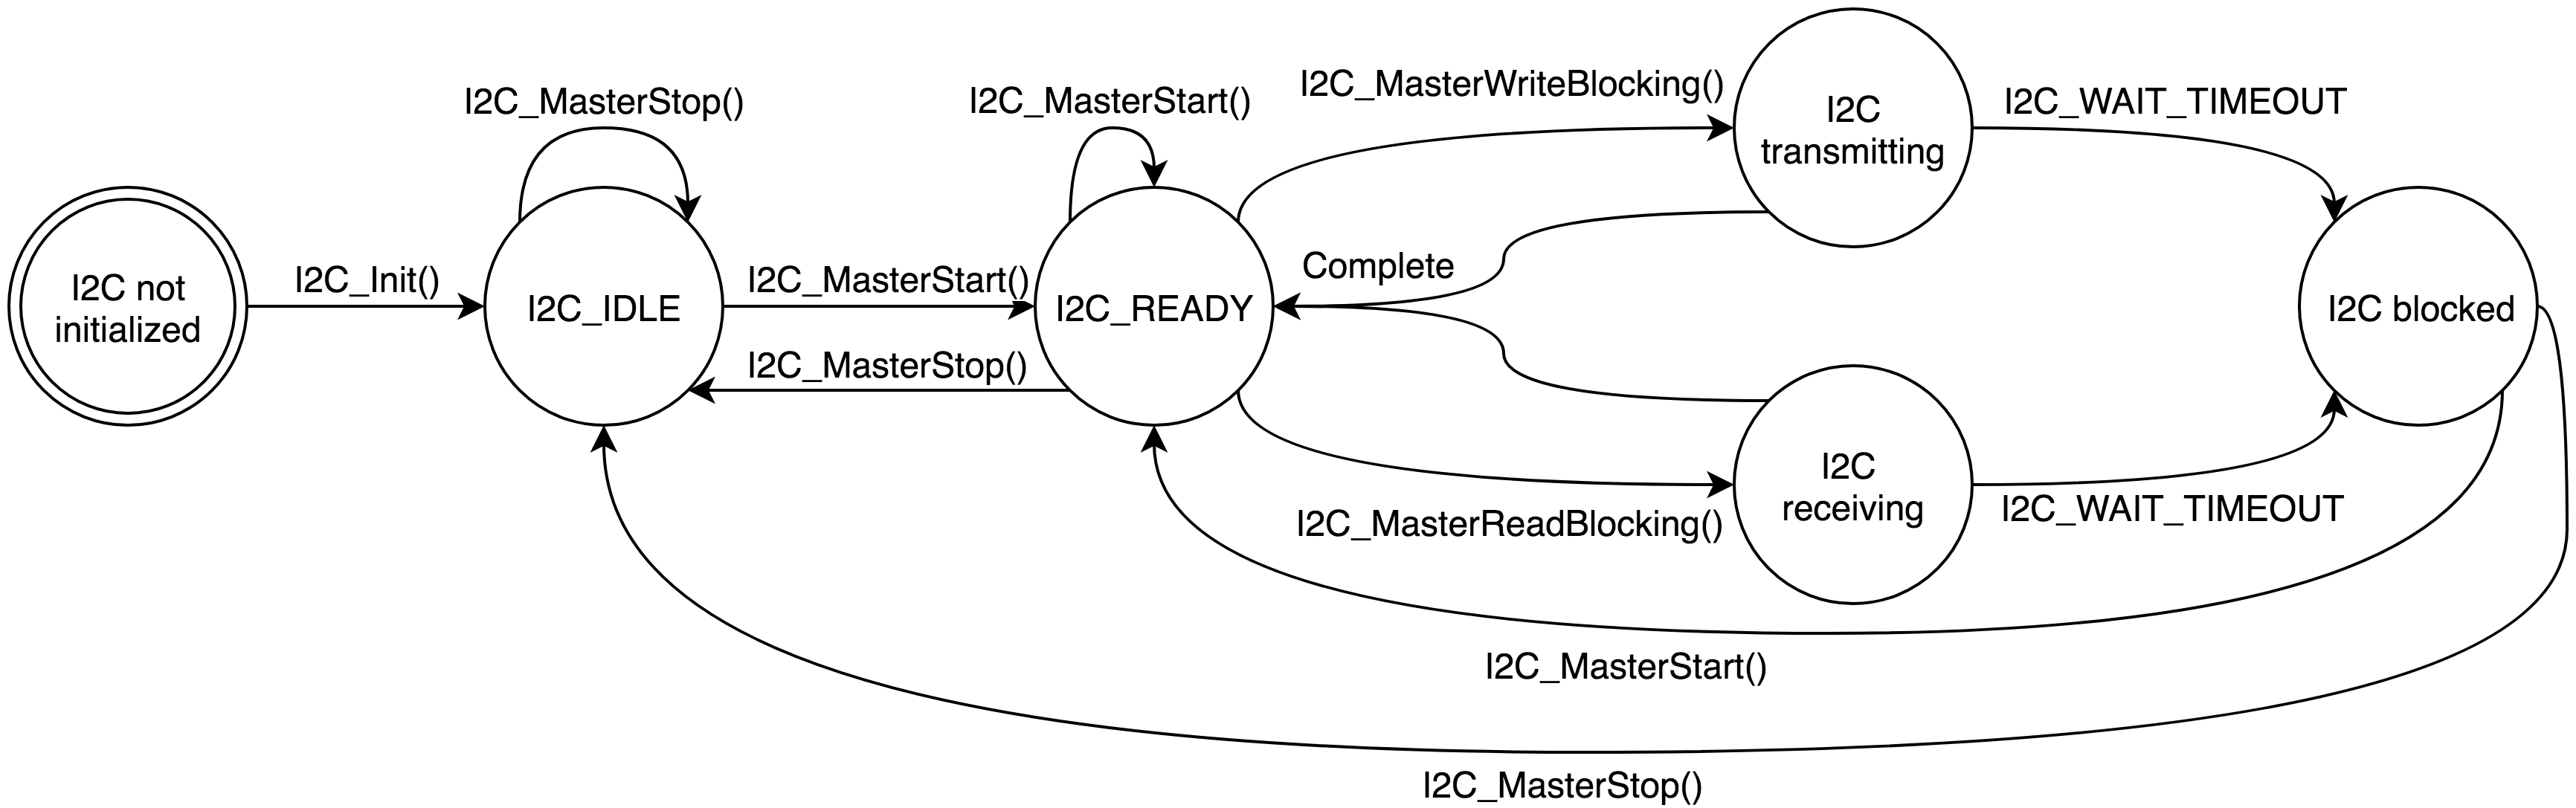
\includegraphics[width=15cm]{billeder/I2C_sm.png}
	\caption{State-machine over I2C driveren}
	\label{fig:I2C_sm}
\end{figure}

På figur \ref{fig:I2C_sm} ses state-machinen over I2C driveren. I2C driveren skal først initialiseres med \verb|I2C_Init()| hvorefter systemet er i idle. Her skal programmet, når nødvendigt, sende en start kommando afhængigt af om systemet skal være \textit{master} eller \textit{slave} (her \textit{master}). Dette gøres med \verb|I2C_MasterStart()| hvorefter I2C er opsat og klar til at sende eller modtage. \\

\verb|I2C_MasterWriteBlocking()| eksekveres når der skal sendes data til slaven. Skulle der ske en fejl på bus'en, vil driveren efter \verb|I2C_WAIT_TIMEOUT| automatisk sende start eller stop kommandoen igen, afhænigt af "fejlkoden". Samme funktionalitet har \verb|I2C_MasterReadBlocking()|, bortset fra at der her først bliver sendt en adresse samt hvilket register der skal læses fra, hvorefter slaven så svarer. \\

\subsection{Universal Asynchronous Receiver/Transmitter (UART)}
Da kommunikation med en host (computer f.eks.) ønskes, er UART kommunikation den foretrukne metode. Her kan der læses statusmeddelelser fra computeren, såsom overstrøm, overtemperatur samt cellespændinger og strømforbrug.

\begin{figure}[h]
	\centering
	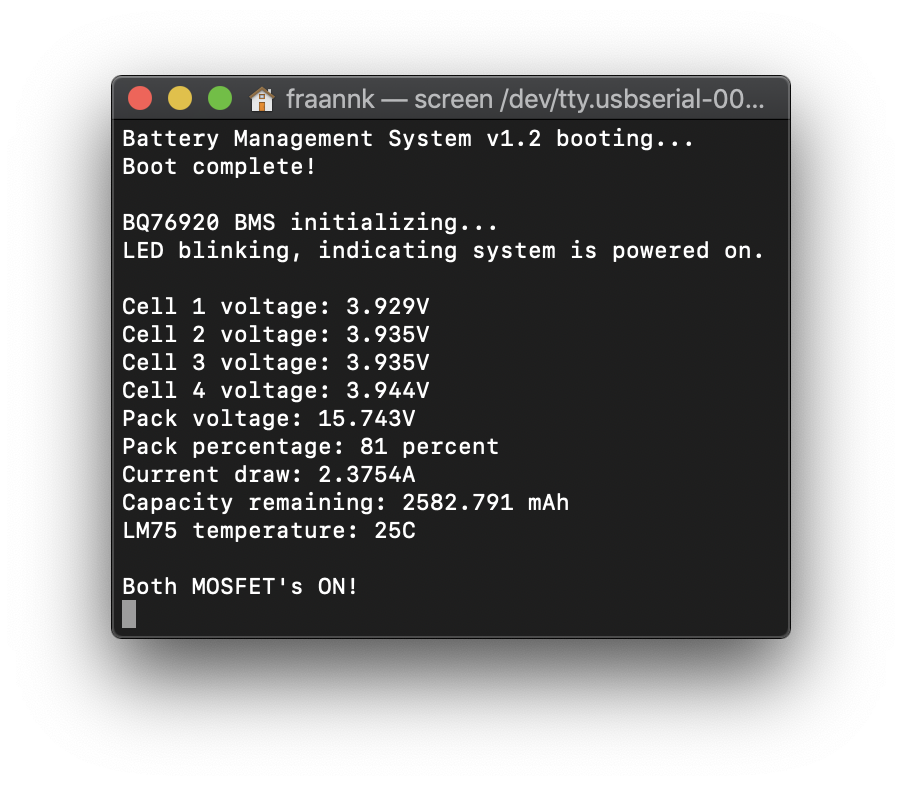
\includegraphics[width=10cm]{billeder/shell_screen.png}
	\caption{Screenshot af Terminal forbundet til BMS'en via UART}
	\label{fig:I2C_sm}
\end{figure}

På host-siden bruges et terminal program (her "Terminal") til at overvåge BMS'en. Cellernes spændinger og aktuelt strømforbrug og andet bliver regelmæssigt overvåget og sendt til host. Shell'en giver også besked hvis brugeren skal foretage sig noget, som f.eks. et reset ved overstrøm.

\begin{figure}[h]
	\centering
	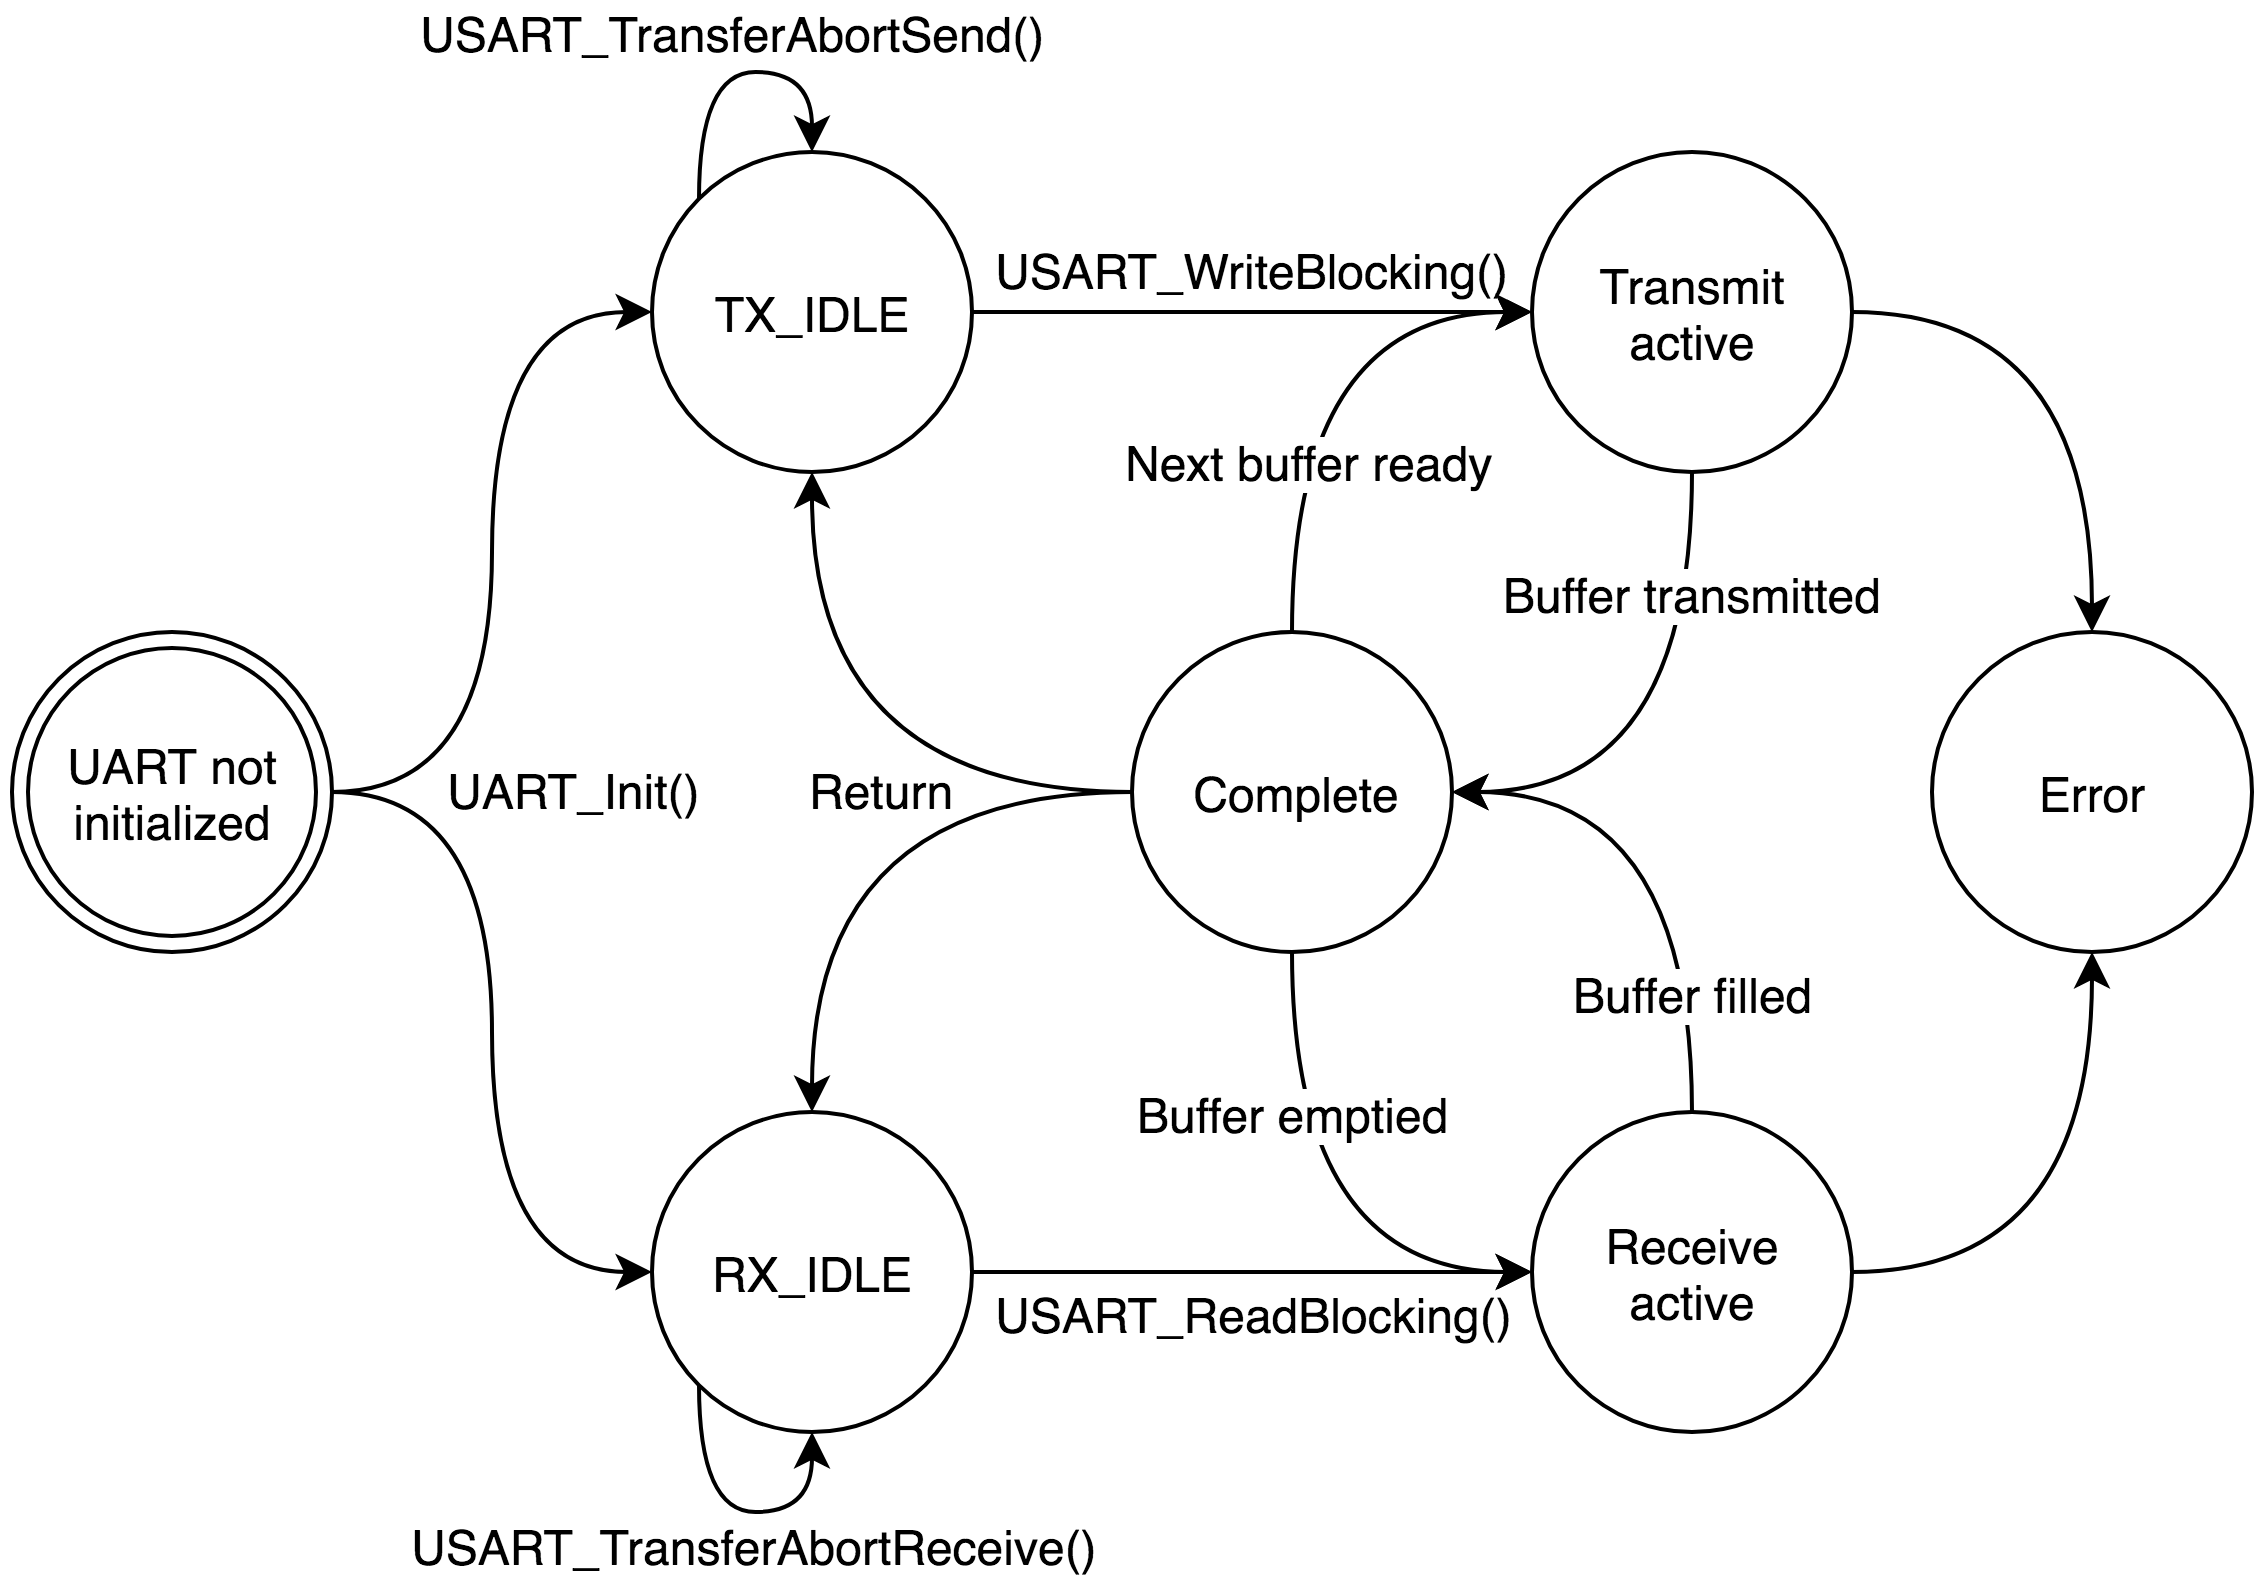
\includegraphics[width=11cm]{billeder/UART_sm.png}
	\caption{State-machine over UART driveren}
	\label{fig:UART_sm}
\end{figure}

På figur \ref{fig:UART_sm} ses state-machinen over U(S)ART driveren.\footnote{Driveren understøtter USART men kun UART bliver brugt.} Her initialiseres driveren med \verb|UART_Init()| og driveren er derefter i idle. Når systemet kalder \verb|USART_WriteBlocking()| (højst sandsynligt gennem \verb|printf()| eller lign.) sender systemet hvad end der befinder sig i bufferen. Når dette er overstået, tjekkes der for eventuelt "genfyldt" buffer, og ellers afsluttes handlingen og returnerer til idle. Det samme sker ved \verb|USART_ReadBlocking()| dog i den modsatte retning. 

\subsection{JTAG}
For at programmere kredsen er der implementeret en variant af en JTAG connector. Denne connector er valgt for at spare plads på boardet, samt at den er billigere i materialer. Igennem denne connector bliver microcontrolleren programmeret ved hjælp af SWD. Her tildeles $\overline{RESET}$, $TDO$, $TDI$, og $TRST$-benene til connectoren. \\

Da denne funktion ikke kræver en decideret opsætning, men derimod en fysisk programmer, er der ikke undersøgt yderligere om dens funktionalitet. Denne funktionalitet anvendes kun under udvilking og produktion, og er derfor ikke noget som brugeren får adgang til. 

\subsection{ALERT pin}
På BMS'en med den integrerede version, sender IC'en et signal til microcontrolleren hver gang der er en status opdatering. Dette signal er et seperat ben som bliver enten logisk højt eller lavt efter hvilken meddelelse der er. Her kan micro'en læse de respektive status-registre for at se nuværende status. Denne funktion er kun anvendt på den integrerede variant af BMS'en, og er noget der er styret alene af IC'en. Microcontrolleren skal via I2C udlæse statusregistrene for at resette dette ben. 
